\documentclass[../../main.tex]{subfiles}
\begin{document}

{\bf[解]}

\begin{figure}[htb]
  \centering
  % 俯角 65°，方位角 115° で見やすい 3D 視点を設定
  \tdplotsetmaincoords{65}{115}
  \begin{tikzpicture}[tdplot_main_coords, scale=2.0, >=stealth, every node/.style={font=\small}]

    % --- 1. 定数・主要点 ---
    % 立体 V: 0 <= z <= 2 - (x^2 + y^2)
    % 底面円の半径 R = sqrt(2) ≈ 1.414
    \def\radR{1.4142}
    \coordinate (O) at (0, 0, 0);

    % 点 P(1, 0, 1) (xz 平面上の接点)
    \coordinate (P) at (1.0, 0, 1.0);

    % --- 2. 座標軸 ---
    \draw[->, thick, gray!70] (-1.8, 0, 0) -- (2.2, 0, 0) node[below right=1pt] {$x$};
    \draw[->, thick, gray!70] (0, -1.8, 0) -- (0, 2.0, 0) node[right=2pt] {$y$};
    \draw[->, thick, gray!70] (0, 0, -0.3) -- (0, 0, 2.7) node[above=2pt] {$z$};
    \node[below left=2pt] at (O) {$O$};

    % --- 3. 立体 V の放物面（薄い透過塗りつぶし）---
    % 放物面の頂点 (0, 0, 2)
    \coordinate (Top) at (0, 0, 2.0);

    % 底面円 z = 0 (半径 sqrt(2))
    \draw[thick, teal!85!black]
    plot[domain=0:360, samples=50] ({\radR*cos(\x)}, {\radR*sin(\x)}, 0);

    % xz 平面内の主断面放物線 (y = 0)
    \draw[very thick, teal!85!black, domain=-\radR:\radR, samples=40]
    plot (\x, 0, {2.0 - \x*\x});

    % yz 平面内の主断面放物線 (x = 0)
    \draw[thick, teal!65!black, domain=-\radR:\radR, samples=40]
    plot (0, \x, {2.0 - \x*\x});

    % --- 4. 等高線 z = 1 (半径 1 の円) ---
    \draw[dashed, gray!60]
    plot[domain=0:360, samples=40] ({1.0*cos(\x)}, {1.0*sin(\x)}, 1.0);

    % --- 5. 点 P(1, 0, 1) と座標投影破線 ---
    % z 軸への投影 (0, 0, 1)
    \draw[dashed, gray!60] (0, 0, 1.0) -- (P);
    \node[left=2pt, font=\scriptsize] at (0, 0, 1.0) {$1$};

    % xy 平面への投影 (1, 0, 0)
    \draw[dashed, gray!60] (P) -- (1.0, 0, 0);
    \node[below=2pt, font=\scriptsize] at (1.0, 0, 0) {$1$};

    % 主要目盛りラベル
    \node[above right=1pt, font=\scriptsize] at (0, 0, 2.0) {$2$};
    \node[below right=1pt, font=\scriptsize] at (\radR, 0, 0) {$\sqrt{2}$};
    \node[above left=1pt, font=\scriptsize] at (-\radR, 0, 0) {$-\sqrt{2}$};

    % 点 P のプロット
    \fill[red!85!black] (P) circle (0.8pt) node[right=3pt, red!90!black, font=\normalsize] {$P(1,0,1)$};
    \fill (Top) circle (0.6pt);

    % --- 6. 点 P における接線/接平面の補助線 (z = -2x + 3) ---
    % xz 平面内での接線 (P を通り傾き -2)
    \draw[thick, blue!85!black] (0.6, 0, 1.8) -- (1.5, 0, 0);
    \fill[blue!85!black] (1.5, 0, 0) circle (0.6pt)
    node[below=2pt, font=\scriptsize, blue!90!black] {$\frac{3}{2}$};

    % % --- 7. 注釈ボックス ---
    % \node[draw=teal!85!black, fill=white, rounded corners=2pt, inner sep=3.5pt, font=\footnotesize, align=left]
    %   at (1.6, -0.6, 2.3) {
    %     \textbf{立体 $V$ と接点 $P$}:\\[2pt]
    %     $\bullet\ V: 0 \le z \le 2-(x^2+y^2)$\\[2pt]
    %     $\bullet\ P(1, 0, 1)$ での接平面:\\[2pt]
    %     \phantom{$\bullet$ } $z = -2x + 3$\\[2pt]
    %     $\bullet\ xy$ 平面 ($z=0$) との交線: $x = \frac{3}{2}$
    %   };

  \end{tikzpicture}
  \caption{立体 $V$（放物面）と接点 $P(1,0,1)$ および接平面の 3D 見取り図}
  \label{fig:paraboloid_tangent_plane}
\end{figure}

題意の立体$V$の方程式は
\begin{align}
  V: 0 \le z \le 2-(x^2+y^2) \label{eq:1}
\end{align}
である．また，対称性から$P(1,0,1)$としてよい．
点$P$での$V$の接平面は$(2-x^2)'=-2x$ゆえ，
\begin{align}
  z=-2x+3 \label{eq:2}
\end{align}
である．

\begin{figure}[htb]
  \centering
  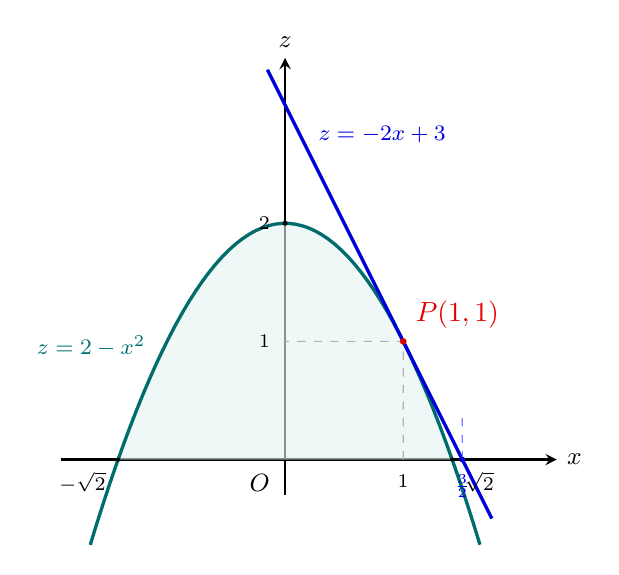
\begin{tikzpicture}[scale=1.5, >=stealth, every node/.style={font=\small}]

    % --- 1. 定数・主要座標 ---
    \def\sqTwo{1.4142} % sqrt(2) ≈ 1.414

    \coordinate (O)     at (0, 0);
    \coordinate (P)     at (1.0, 1.0);      % 接点 P(1, 1)
    \coordinate (X_int) at (1.5, 0);        % 接線と z=0 の交点 (3/2, 0)
    \coordinate (Z_top) at (0, 2.0);        % 放物線の頂点 (0, 2)
    \coordinate (Z_int) at (0, 3.0);        % 接線の z 切片 (0, 3)

    % --- 2. 座標軸 ---
    \draw[->, thick] (-1.9, 0) -- (2.3, 0) node[right] {$x$};
    \draw[->, thick] (0, -0.3) -- (0, 3.4) node[above] {$z$};
    \node[below left=2pt] at (O) {$O$};

    % --- 3. 放物線 z = 2 - x^2 (y = 0) ---
    % 切断面の内部（薄い透過塗りつぶし）
    \fill[teal!10, opacity=0.6, domain=-\sqTwo:\sqTwo, samples=50]
    (-\sqTwo, 0) -- plot (\x, {2.0 - \x*\x}) -- (\sqTwo, 0) -- cycle;

    % 放物線の描画
    \draw[very thick, teal!85!black, domain=-1.65:1.65, samples=60]
    plot (\x, {2.0 - \x*\x});
    \node[teal!90!black, font=\footnotesize, above left] at (-1.1, 0.79) {$z = 2 - x^2$};

    % --- 4. 接線 z = -2x + 3 (接平面の断面) ---
    \draw[very thick, blue!85!black] (-0.15, 3.3) -- (1.75, -0.5);
    \node[blue!90!black, font=\footnotesize, above right] at (0.2, 2.6) {$z = -2x + 3$};

    % --- 5. 点 P(1, 1) と座標投影破線 ---
    \draw[dashed, gray!60] (1.0, 0) -- (P) -- (0, 1.0);
    \node[below=2pt, font=\scriptsize] at (1.0, 0) {$1$};
    \node[left=2pt, font=\scriptsize]  at (0, 1.0) {$1$};

    % 接線の x 切片 (3/2, 0)
    \draw[dashed, blue!50] (X_int) -- (1.5, 0.4);
    \fill[blue!85!black] (X_int) circle (0.7pt)
    node[below=2pt, font=\scriptsize, blue!90!black] {$\frac{3}{2}$};

    % 放物線の x 切片 (±sqrt(2)) と頂点 (0, 2)
    \fill (Z_top) circle (0.6pt) node[left=2pt, font=\scriptsize] {$2$};
    \fill (\sqTwo, 0) circle (0.5pt) node[below right=1pt, font=\scriptsize] {$\sqrt{2}$};
    \fill (-\sqTwo, 0) circle (0.5pt) node[below left=1pt, font=\scriptsize] {$-\sqrt{2}$};

    % 接点 P のプロット
    \fill[red!85!black] (P) circle (0.8pt)
    node[above right=1pt, red!90!black, font=\normalsize] {$P(1, 1)$};

    % % --- 6. 注釈ボックス ---
    % \node[draw=blue!85!black, fill=white, rounded corners=2pt, inner sep=3.5pt, font=\footnotesize, align=left]
    %   at (-1.1, 2.5) {
    %     \textbf{$y=0$ における切断面}:\\[2pt]
    %     $\bullet$ 放物線: $z = 2 - x^2$\\[2pt]
    %     $\bullet$ 接線: $z' = -2x \implies z = -2(x-1) + 1$\\[2pt]
    %     \phantom{$\bullet$ 接線: } $\therefore z = -2x + 3$\\[2pt]
    %     $\bullet$ $z = 0$ との交点: $x = \dfrac{3}{2}$
    %   };

  \end{tikzpicture}
  \caption{$y=0$（$xz$ 平面）における切断面：放物線 $z=2-x^2$ と接点 $P(1,1)$ における接線}
  \label{fig:xz_plane_tangent_cut}
\end{figure}

よって$xy$平面($z=0$)では$x=\dfrac{3}{2}$となり，
$xy$平面での円$C$と接平面の断面図は以下のようになる．

\begin{figure}[htb]
  \centering
  \begin{tikzpicture}[scale=1, >=stealth, every node/.style={font=\small}]

    % --- 1. パラメータ定義 ---
    % 解より r = 3, theta = pi/3 = 60°
    % x = r * cos(60°) = 1.5 = 3/2
    \def\radR{3.0}
    \def\angTheta{60}
    \def\xCut{1.5}

    \coordinate (O) at (0, 0);

    % 直線 x = 3/2 と円 C の交点
    \coordinate (P_top) at (\xCut, {\radR * sin(\angTheta)});
    \coordinate (P_bot) at (\xCut, {-\radR * sin(\angTheta)});

    % --- 2. 座標軸 ---
    \draw[->, thick] (-0.5, 0) -- (3.8, 0) node[right] {$x$};
    \draw[->, thick] (0, -3.2) -- (0, 3.2) node[above] {$y$};
    \node[below left=2pt] at (O) {$O$};

    % --- 3. 円 C の描画 ---
    % 影の部分 (細い実線)
    \draw[thick, gray!70]
    (\angTheta:\radR) arc[start angle=\angTheta, end angle={360-\angTheta}, radius=\radR];

    % 光が当たる部分 (x >= 3/2 の円弧: 太線強調)
    \draw[line width=2.0pt, blue!85!black]
    (-\angTheta:\radR) arc[start angle=-\angTheta, end angle=\angTheta, radius=\radR];
    \node[blue!90!black, font=\normalsize, right=3pt] at (150:\radR) {$C$};

    % --- 4. 接平面の交線 (直線 x = 3/2) ---
    \draw[thick, red!80!black] (\xCut, -3.0) -- (\xCut, 3.0);
    \node[below right=1pt, red!85!black, font=\scriptsize] at (\xCut, 0) {$\frac{3}{2}$};

    % --- 5. 動径 r と角度 theta ---
    \draw[thick, black] (O) -- (P_top);
    \node[above left=1pt] at ($ (O)!0.55!(P_top) $) {$r$};

    % 角度 theta の弧
    \draw[thick, purple!85!black] (0.6, 0) arc[start angle=0, end angle=\angTheta, radius=0.6];
    \node[purple!90!black, font=\footnotesize] at (30:0.85) {$\theta$};

    % --- 6. 主要点のプロット ---
    \fill (O) circle (0.7pt);
    \fill[red!85!black] (P_top) circle (0.9pt);
    \fill[red!85!black] (P_bot) circle (0.9pt);

    % % --- 7. 注釈ボックス ---
    % \node[draw=blue!85!black, fill=white, rounded corners=2pt, inner sep=3.5pt, font=\footnotesize, align=left]
    %   at (2.5, -2.2) {
    %     \textbf{光が当たる部分}:\\[2pt]
    %     $\bullet\ x \ge \dfrac{3}{2}$（太線部）\\[2pt]
    %     $\bullet\ \text{弧長} = 2r\theta = 2\pi$\\[2pt]
    %     $\bullet\ r\cos\theta = \dfrac{3}{2}$
    %   };

  \end{tikzpicture}
  \caption{$xy$ 平面における円 $C$ と接平面の交線 $x = \dfrac{3}{2}$（太線部は光が当たる領域）}
  \label{fig:xy_plane_cut}
\end{figure}

よって円$C$のうち光が当たる部分は$3/2\le x$である．
$C$の半径$r_{>0}$とし，上図のように$\theta $($0<\theta<\pi/2$)をおく．
題意より，上図で太線の部分の長さが$2\pi$だから
\begin{align}
  2r\theta=2\pi \label{eq:3}
\end{align}
である．また，$r,\theta$の関係は図から
\begin{align}
  r\cos t=\dfrac{3}{2} \label{eq:4}
\end{align}
である．\cref{eq:1,eq:2}から$r$を消去して
\begin{align}
  \dfrac{2\pi}{3}=\dfrac{\theta}{\cos \theta}
\end{align}
である．

この右辺は$0<t<\pi/2$で単調増加な関数の積だから単調増加である．
加えて$\theta=\pi/3$が解であることから，これが唯一の解である．
この時\cref{eq:4}から$r=3$となり，求める影の長さは
\begin{align}
  (2\pi-2\theta)r=4\pi
\end{align}
である．$\cdots$(答)

\newpage
\end{document}
